\documentclass[a4paper,12pt]{article}

\usepackage[margin=1in]{geometry}
\usepackage{xcolor}
\usepackage{graphicx}
\usepackage{amssymb}

\title{\texttt{Binary Number Systems}\\\hrulefill}
\author{Digital Electronics | Lecture 2}
\date{8/23/2023}

\begin{document}
    \maketitle

    \section*{Intro}
    
    \begin{itemize}
        \item Software (typically from a high level programming langauge), abstracts certain computational functions to make writing code more feasible
        \item the next step will be the assembly process, written in pure references of transistor processes
        \item transistor switching 
    \end{itemize}
    \section*{Binary Numer Systems}
    there are three types of number systems $\rightarrow$ \texttt{Decimal, Binary, Hexadecimal}

    \subsection*{Bits}
        A \textbf{bit} is simply a single binary value. These are the followin notations for increases in the number of bits.
        \begin{itemize}
            \item 8 bit $\rightarrow$ 1 byte
            \item 16 bits $\rightarrow$ 1 words, 2 bytes
            \item 32 bits $\rightarrow$ 2 words, 4 bytes (floats)
            \item 64 bits $\rightarrow$ 2 longs, 4 words, 8 bytes (double in programming)
        \end{itemize}
        64 bits are usually called a \texttt{long long} in hardware. Additionally, B $\rightarrow$ bytes 8B is 8 btes, and b $\rightarrow$ bits, 4b is 4 bits.
        \par $2^n$, where n is the number os bits, is the number of possible values that could be represented by said number of bits. This entails
        \begin{itemize}
            \item Min and max number a binary 
            \item possible input combination to a digital circuit
        \end{itemize}

        \section*{Number System}
        Numbers in everyday use are reffered to as decimal Numbers
        \[7,392=(7*10^3)+(3*10^2)+(9*10^1)+(2*10^0)\]
        Value of \# = $V_0(B^d)+V_0(B^d)+V_0(B^d)...$ where V is the value of a digit, B is the base, and d is the digit's place.\par 
        Binary systems are base 2, only compirsed of the value 1 \& 0. Hexadecimal an doctal numvers are base 16 and 8 respectively. Hex digits have 16 values, and octal digits have 8 values. \par
        Subscripts to the right most of a digit denotes its base.
        \begin{itemize}
            \item $1101_{10}$ $\rightarrow$ base 10
            \item $1101_{2}\rightarrow$ base 2 
        \end{itemize}

        \subsection*{Converting Binary to decimal}
        Raise the value to the power of it's place.
        10011011 $\downarrow$ [$V_0(B^d)+V_0(B^d)+V_0(B^d)...$]
        \[2^7*1+2^6*0+2^5*0+2^4*1+2^3*1+2^2*0+2^1*1+2^0*1\]
        \begin{itemize}
            \item \texttt{LSB} $\rightarrow$ least Siginficant Bit
            \item \texttt{MSB} $\rightarrow$ Most Siginficant Bit
        \end{itemize}
        *If the LSB is 1, the decimal number is odd, if 0 it's even.

        \subsection*{Converting Decimal to Binary}
            \begin{itemize}
                \item Divide decimal number by 2 and remainder is binary value
                \item continue to divide result by 2 using remainder as binary value
                \item stop when no more division can occur
            \end{itemize}
            10: 10/2 = 0 (LSB), 5/2 = 1, 2/2 = 0, 1/2 = 1

        \section*{Hexidecimal}
        \begin{minipage}{8cm}
            Hex is a convenient way of expressing very large Numbers. One digit is 4 bits and the digits range from 0 - F (16 values). A 0x prefix denotes a Hex value (0x90FBE).    
        \end{minipage}
        \hspace{20pt}
        \begin{minipage}{10cm}
            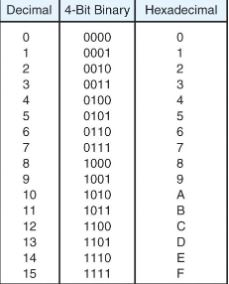
\includegraphics[width=5cm]{Hex tables.JPG}
        \end{minipage}
        \subsection*{Converting between Decimal, Binary, and Hex} 
        \begin{minipage}{10cm}
            \begin{itemize}
                \item split the Binary number into groups of four, padding any remaining space with 0s
                \item replace them with their corresponding Hex value (table will be provided during assessments)
            \end{itemize}
        \end{minipage}
        \hspace{0.05\textwidth}
        \begin{minipage}{10cm}
            ~~101111\\0010~~~1111\\~~~2~~~~~F\\0x2F
        \end{minipage}
        \vspace{12pt}
        \par Converting from Decimal to Hex is just that process but in reverse, or you can use the \texttt{remainder divisor method} with \textbf{16} as the base (LSB$\rightarrow$MSB).\\\textbf{Given 590} \[\frac{590}{16}=36~r~14(E),~\frac{36}{16}=2~r~4,~\frac{2}{16}=0~r~2\] \[\therefore~590_{10}=0\textnormal{x}24\textnormal{E}\]
        This process reversed yeilds \texttt{Hexadecimal}$~\rightarrow~$\texttt{Decimal}.

        \subsection*{Octal}
        \begin{minipage}{9cm}
            Octal is a predecesor to Hex, representing 8 possible values (0-7) within each digit. It was useful in the era of data being stored in multiples of 3 (3 bits represent one octal digit).\[1111\rightarrow001~~111\rightarrow1~~7\rightarrow17_8\]  
        \end{minipage}
        \hspace{20pt}
        \begin{minipage}{9cm}
            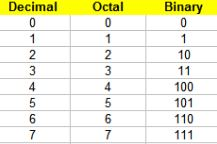
\includegraphics{Octal table.JPG}
        \end{minipage}
        \vspace{20pt}$\rightarrow$\textbf{LSB}\\\textbf{Given 370} \[\frac{370}{8}=46~r~2,~\frac{46}{8}=5~r~6,~\frac{5}{8}=0~r~5\] \[\therefore~370_{10}=562_8\]
\end{document}